\chapter{Arhitektura i dizajn sustava}
		
		\textbf{\textit{dio 1. revizije}}\\

		\textit{ Potrebno je opisati stil arhitekture te identificirati: podsustave, preslikavanje na radnu platformu, spremišta podataka, mrežne protokole, globalni upravljački tok i sklopovsko-programske zahtjeve. Po točkama razraditi i popratiti odgovarajućim skicama:}
	\begin{itemize}
		\item 	\textit{izbor arhitekture temeljem principa oblikovanja pokazanih na predavanjima (objasniti zašto ste baš odabrali takvu arhitekturu)}
		\item 	\textit{organizaciju sustava s najviše razine apstrakcije (npr. klijent-poslužitelj, baza podataka, datotečni sustav, grafičko sučelje)}
		\item 	\textit{organizaciju aplikacije (npr. slojevi frontend i backend, MVC arhitektura) }		
	\end{itemize}
	
	Od mogućih arhitektura sustava, za svoj projekt smo odabrali objektno usmjerenu arhitekturu. Tu arhitekturu smo odabrali zato što se koristi u industriji te je defacto standard razvoja programskih rješenja. Osim toga, ona je fleksibilna i pregledna, što nam je bitno s obzirom na to da više ljudi radi na implementaciji aplikacije. Zahvaljujući modularnosti programskog rješenja, greške su lako ispravljive, a nove mogućnosti se lako dodaju od bilo strane koje osobe u timu.\\

	Odlučili smo se za web aplikaciju, koja je prilagođena mobilni uređajima, obzirom da glazbenici, a time i bendovi nemaju uvijek pristup računalu, a ne želimo da je korisnik ograničen samo na mobilne uređaje.\\

	Arhitekturu sustava možemo podijeliti na tri podsustava:
		\begin{itemize}
			\item Web preglednik
			\item Web poslužitelj
    			\item Web aplikacija
			\item Baza podataka
		\end{itemize}


	Korisnik (javnost, glazbenik, bend, administrator) pristupa web aplikaciji uz pomoć svog web preglednika, s time da se u sredini nalazi web poslužitelj. Na njemu se nalazi aplikacija koju on pokreće, te uz pomoć protokola komunicira s korisnicima.\\

	Klijentski(frontend) dio aplikacije omogućuje da korisnik korištenjem sučelja može pristupiti serveru(backend) aplikacije. Ovisno o tome što korisnik hoće, taj server ima mogućnost spajanja na bazu podataka kako bi korisniku prikazao informacije.\\

	Backend je napisan u Javi, a kao razvojni okvir koristimo Java Spring Boot. Dodani su projekti Spring Data kako bi backend mogao lako komunicirati s bazom, Spring Web MVC za rukovanje sa request-ima te Spring Security kako bi zaštitili aplikaciju od vanjskih napada. \\

	\begin{figure}[H]
		\begin{center}
			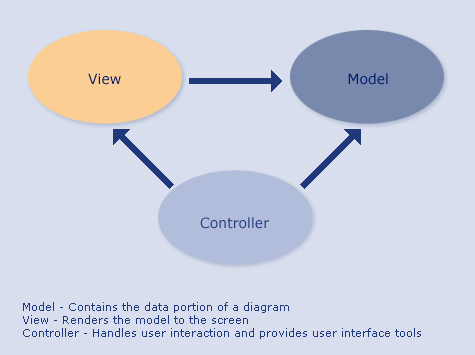
\includegraphics[width=10cm]{slike/mvc.PNG}
		\end{center}
		\caption{Pojednostavljeni prikaz MVC-a}
		\label{fig:mvc}
	\end{figure}

	Za frontend koristimo React. On je moderni i jednostavan framework koji koristi HTML, CSS, JSX i JavaScript uz pomoć kojeg smo napravili sučelje za našu aplikaciju. Uz pomoć React-a možemo lagano komunicirati s backendom koristeći REST.\\




		\section{Baza podataka}
			
			\textbf{\textit{dio 1. revizije}}\\
			
		\textit{Potrebno je opisati koju vrstu i implementaciju baze podataka ste odabrali, glavne komponente od kojih se sastoji i slično.}
		
		Za potrebe razvoja \textit{Gigera} koristit će se objektno relacijsko mapiranje. To je metoda koja se koristi u objektno-orijentiranim jezicima te se na taj način stvara virtualna objektna baza podataka.
		
		Baza podataka sastoji se od sljedećih entiteta:
		
		\begin{packed_item}
		\item Comment
		\item Message
		\item Conversation
		\item Conversation\_user
		\item System\_person
		\item People
		\item System\_person\_roles
		\item Organizer
		\item Conversation\_band
		\item Band
		\item Gig\_type
		\item Band\_occasions
		\item Occasion
		\item Musician\_occasions
		\item Band\_invited\_back\_up\_members
		\item Band\_invited
		\item Band\_back\_up\_members
		\item Musician\_bands
		\item Post
		\item Musician
		\item Instruments
		\item Instrument
		\item Musician\_gig\_history
		\item Gig
		\item Review\_gig
		\item Review
		
	\end{packed_item}
	
	
	
	\subsection{Opis tablica}
	
	\begin{longtabu} to \textwidth {|X[6, l+3]|X[6, l]|X[20, l]|}
		
		\hline \multicolumn{3}{|c|}{\textbf{Comment}}	 \\[3pt] \hline
		\endfirsthead
		
		\hline 
		\endlastfoot
		
		\textbf{id} & BIGINT	&  	jedinstveni identifikator komentara 	\\ \hline
		content & VARCHAR & sadržaj komentara \\ \hline
		posted\_on & TIMESTAMP & datum i vrijeme objave komentara \\ \hline	
		\textit{author\_id} & BIGINT & jedinstveni identifikator autora komentara \\ \hline
		\textit{fk\_post} & BIGINT & jedinstveni identifikator komentara \\ \hline
		
	\end{longtabu}
	
	\textit{\bf Message}
	\textit{Ovaj entitet sadrži informacije o poruci. Sadrži atribute: id poruke, sadržaj poruke, vrijeme kada je poruka poslana, id pošiljatelja i id razgovora. Ovaj entitet je u \emph{Many-to-Many} vezi  sa entitetom Message\_seen te je u \emph{Many-to-many} vezi sa entitetima Conversation i User.}
	\begin{longtabu} to \textwidth {|X[6, l+3]|X[6, l]|X[20, l]|}
		
		\hline \multicolumn{3}{|c|}{\textbf{Message}}	 \\[3pt] \hline
		\endfirsthead
		
		\hline
		\endlastfoot
		
		\textbf{id} & BIGINT	&  	jedinstveni identifikator poruke 	\\ \hline
		content	& VARCHAR & sadržaj poruke	\\ \hline
		sent\_time & TIMESTAMP & vrijeme kada je poruka poslana \\ \hline
		\textit{fk\_sender} & BIGINT & jedinstveni identifikator pošiljatelja \\ \hline
		\textit{fk\_sender\_band} & BIGINT & jedinstveni identifikator benda pošiljatelja \\ \hline
		\textit{fk\_converation} & BIGINT & jedinstveni identifikator razgovora \\ \hline
		
	\end{longtabu}
	
	\textit{\bf Conversation}
	\textit{Ovaj entitet sadrži informacije o razgovoru. Sadrži atribute: id razgovora i ime razgovora. Ovaj entitet je u \emph{One-to-Many} vezi  sa entitetima:Message i Conversation\_user.}
	\begin{longtabu} to \textwidth {|X[6, l+3]|X[6, l]|X[20, l]|}
		
		\hline \multicolumn{3}{|c|}{\textbf{Conversation}}	 \\[3pt] \hline
		\endfirsthead
		
		\hline
		\endlastfoot
		
		\textbf{id} & BIGINT	&  	jedinstveni identifikator razgovora 	\\ \hline
		\textit{fk\_band} & BIGINT & jedinstveni identifikator benda \\ \hline
		picture\_url & VARCHAR & url slike razgovora \\ \hline
		title	& VARCHAR &  naziv razgovora	\\ \hline
		
	\end{longtabu}
	
	\textit{\bf Conversation\_user}
	\textit{Ovaj entitet sadrži informacije o korisniku u razgovoru. Sadrži atribute: id korisnika i id razgovora. Ovaj entitet je u \emph{Many-to-One} vezi  sa entitetima:User i Conversation.}
	\begin{longtabu} to \textwidth {|X[6, l+3]|X[6, l]|X[20, l]|}
		
		\hline \multicolumn{3}{|c|}{\textbf{Conversation\_user}}	 \\[3pt] \hline
		\endfirsthead
		
		\hline
		\endlastfoot
		
		\textit{fk\_user} & BIGINT	&  	jedinstveni identifikator korisnika	\\ \hline
		\textit{fk\_conversation}	& BIGINT &  jedinstveni identifikator razgovora	\\ \hline
		
	\end{longtabu}
	
	
	\begin{longtabu} to \textwidth {|X[6, l+3]|X[6, l]|X[20, l]|}
		
		\hline \multicolumn{3}{|c|}{\textbf{System\_person}}	 \\[3pt] \hline
		\endfirsthead
		
		\hline
		\endlastfoot
		
		\textbf{id} & BIGINT	&  	jedinstveni identifikator sustavskih podataka o korisniku	\\ \hline
		email & VARCHAR & email adresa osobe \\ \hline
		locked & BOOLEAN & korisnik ima zabranu korištenja aplikacije ili ne \\ \hline
		password\_hash & VARCHAR & hash lozinke osobe \\ \hline
		verified & BOOLEAN & email adresa potvrđena ili ne \\ \hline
		
	\end{longtabu}
	
	\begin{longtabu} to \textwidth {|X[6, l+3]|X[6, l]|X[20, l]|}
		
		\hline \multicolumn{3}{|c|}{\textbf{Person}}	 \\[3pt] \hline
		\endfirsthead
		
		\hline
		\endlastfoot
		
		\textbf{id} & BIGINT	&  	jedinstveni identifikator korisnika	\\ \hline
		phone\_number & VARCHAR & telefonski broj korisnika \\ \hline
		picture\_url & VARCHAR & url slike korisnika \\ \hline
		username & VARCHAR & korisničko ime korisnika
		
	\end{longtabu}
	
	\begin{longtabu} to \textwidth {|X[6, l+3]|X[6, l]|X[20, l]|}
		
		\hline \multicolumn{3}{|c|}{\textbf{System\_person\_roles}}	 \\[3pt] \hline
		\endfirsthead
		
		\hline
		\endlastfoot
		
		\textbf{system\_person\_id} & BIGINT	&  	jedinstveni identifikator sustavskih podataka o korisniku	\\ \hline
		roles & INT & Uloga korisnika \\ \hline
		
		
	\end{longtabu}
	
	\textit{\bf Organizer}
	\textit{Ovaj entitet sadrži informacije za organizatora. Sadrži atribute: id organizatora te ime organizatora. Ovaj entitet je u \emph{One-to-Many} vezi  sa entitetima: Review\_organizer, Gig i User}
	\begin{longtabu} to \textwidth {|X[6, l+3]|X[6, l]|X[20, l]|}
		
		\hline \multicolumn{3}{|c|}{\textbf{Organizer}}	 \\[3pt] \hline
		\endfirsthead
		
		\hline
		\endlastfoot
		
		\textbf{id} & BIGINT	&  	jedinstveni identifikator organizatora 	\\ \hline
		manager\_name	& VARCHAR &  ime organizatora	\\ \hline
		
	\end{longtabu}
	
	\begin{longtabu} to \textwidth {|X[6, l+3]|X[6, l]|X[20, l]|}
		
		\hline \multicolumn{3}{|c|}{\textbf{Conversation\_band}}	 \\[3pt] \hline
		\endfirsthead
		
		\hline
		\endlastfoot
		
		\textit{fk\_band} & BIGINT	&  	jedinstveni identifikator benda	\\ \hline
		\textit{fk\_conversation}	& BIGINT &  jedinstveni identifikator razgovora	\\ \hline
		
	\end{longtabu}
	
	\begin{longtabu} to \textwidth {|X[6, l+3]|X[6, l]|X[20, l]|}
		
		\hline \multicolumn{3}{|c|}{\textbf{Band}}	 \\[3pt] \hline
		\endfirsthead
		
		\hline 
		\endlastfoot
		
		\textbf{id} & BIGINT	&  	jedinstveni identifikator benda 	\\ \hline
		bio & VARCHAR & opis benda \\ \hline
		formed\_date & DATE & datum osnutka benda \\ \hline
		address & VARCHAR & adresa benda \\ \hline
		extra\_description & VARCHAR & dodatak opis benda \\ \hline
		x & DOUBLE & x koordinata lokacije \\ \hline
		y & DOUBLE & y koordinata lokacije \\ \hline
		max\_distance & DOUBLE & najveća udaljenost koju bend želi prijeći zbog gaže \\ \hline
		name & VARCHAR & ime benda \\ \hline
		picture\_url & VARCHAR & url slike benda \\ \hline
		\textit{leader\_id}	& BIGINT &  jedinstveni identifikator voditelja benda	\\ \hline 	
		
	\end{longtabu}
	
	\begin{longtabu} to \textwidth {|X[6, l+3]|X[6, l]|X[20, l]|}
		
		\hline \multicolumn{3}{|c|}{\textbf{Gig\_type}}	 \\[3pt] \hline
		\endfirsthead
		
		\hline 
		\endlastfoot
		
		\textbf{gig} &  BIGINT	&  	jedinstveni identifikator vrste nastupa 	\\ \hline
		gig\_type	& VARCHAR &  vrsta nastupa	\\ \hline 		
		
	\end{longtabu}
	
	\begin{longtabu} to \textwidth {|X[6, l+3]|X[6, l]|X[20, l]|}
		
		\hline \multicolumn{3}{|c|}{\textbf{Band\_occasions}}	 \\[3pt] \hline
		\endfirsthead
		
		\hline 
		\endlastfoot
		
		\textit{occasion\_id} &  BIGINT	&  	jedinstveni identifikator događaja 	\\ \hline
		\textit{band\_id} &  BIGINT	&  	jedinstveni identifikator benda koji sudjeluje na događaju 	\\ \hline 		
		
	\end{longtabu}
	
	\begin{longtabu} to \textwidth {|X[6, l+3]|X[6, l]|X[20, l]|}
		
		\hline \multicolumn{3}{|c|}{\textbf{Occasion}}	 \\[3pt] \hline
		\endfirsthead
		
		\hline 
		\endlastfoot
		
		\textbf{id} &  BIGINT	&  	jedinstveni identifikator događaja 	\\ \hline
		description & VARCHAR & opis događaja \\ \hline
		local\_date & DATE & datum održavanja događaja \\ \hline
		personal\_occasion & BOOLEAN & privatan događaj ili ne \\ \hline
		\textit{band\_id} & BIGINT & jedinstveni identifikator benda koji sudjeluje na događaju
		
		
	\end{longtabu}
	
	\begin{longtabu} to \textwidth {|X[6, l+3]|X[6, l]|X[20, l]|}
		
		\hline \multicolumn{3}{|c|}{\textbf{Musician\_occasions}}	 \\[3pt] \hline
		\endfirsthead
		
		\hline 
		\endlastfoot
		
		\textit{musician\_id} &  BIGINT	&  	jedinstveni identifikator glazbenika 	\\ \hline
		\textit{occasions\_id} &  BIGINT	&  	jedinstveni identifikator događaja	\\ \hline
		
		
	\end{longtabu}
	
	\begin{longtabu} to \textwidth {|X[6, l+8]|X[6, l]|X[20, l]|}
		
		\hline \multicolumn{3}{|c|}{\textbf{Band\_invited\_back\_up\_members}}	 \\[3pt] \hline
		\endfirsthead
		
		\hline 
		\endlastfoot
		
		\textit{band\_id} &  BIGINT	&  	jedinstveni identifikator benda 	\\ \hline
		\textit{invited\_back\_up\_members\_id} &  BIGINT	&  	jedinstveni identifikator glazbenika pozvanih u bend kao rezerva	\\ \hline
		
		
	\end{longtabu}
	
	\begin{longtabu} to \textwidth {|X[6, l+3]|X[6, l]|X[20, l]|}
		
		\hline \multicolumn{3}{|c|}{\textbf{Band\_invited}}	 \\[3pt] \hline
		\endfirsthead
		
		\hline 
		\endlastfoot
		
		\textit{band\_id} &  BIGINT	&  	jedinstveni identifikator benda 	\\ \hline
		\textit{invited\_id} &  BIGINT	&  	jedinstveni identifikator glazbenika pozvanih u bend	\\ \hline
		
		
	\end{longtabu}
	
	\begin{longtabu} to \textwidth {|X[6, l+8]|X[6, l]|X[20, l]|}
		
		\hline \multicolumn{3}{|c|}{\textbf{Band\_back\_up\_members}}	 \\[3pt] \hline
		\endfirsthead
		
		\hline 
		\endlastfoot
		
		\textit{band\_id} &  BIGINT	&  	jedinstveni identifikator benda 	\\ \hline
		\textit{invited\_back\_up\_members\_id} &  BIGINT	&  	jedinstveni identifikator glazbenika koji su rezervni članovi	\\ \hline
		
		
	\end{longtabu}
	
	\begin{longtabu} to \textwidth {|X[6, l+3]|X[6, l]|X[20, l]|}
		
		\hline \multicolumn{3}{|c|}{\textbf{Musician\_bands}}	 \\[3pt] \hline
		\endfirsthead
		
		\hline 
		\endlastfoot
		
		\textit{fk\_musician} & BIGINT	&  	jedinstveni identifikator glazbenika 	\\ \hline
		\textit{fk\_band}	& BIGINT &  jedinstveni identifikator benda	\\ \hline 		
		
	\end{longtabu}
	
	\begin{longtabu} to \textwidth {|X[6, l+3]|X[6, l]|X[20, l]|}
		
		\hline \multicolumn{3}{|c|}{\textbf{Post}}	 \\[3pt] \hline
		\endfirsthead
		
		\hline 
		\endlastfoot
		
		\textbf{id} & BIGINT	&  	jedinstveni identifikator objave 	\\ \hline
		content & VARCHAR & sadržaj objave \\ \hline
		published\_on & TIMESTAMP & datum i vrijeme objave objave \\ \hline	
		\textit{fk\_band} & BIGINT & jedinstveni identifikator benda \\ \hline
		\textit{fk\_user} & BIGINT & jedinstveni identifikator korisnika koji je napisao objavu \\ \hline
		
	\end{longtabu}
	
	\begin{longtabu} to \textwidth {|X[6, l+3]|X[6, l]|X[20, l]|}
		
		\hline \multicolumn{3}{|c|}{\textbf{Musician}}	 \\[3pt] \hline
		\endfirsthead
		
		\hline 
		\endlastfoot
		
		bio	& VARCHAR &  opis glazbenika	\\ \hline 
		public\_calendar & BOOLEAN & kalendar glazbenika javan ili ne \\ \hline
		\textbf{id} & BIGINT	&  	jedinstveni identifikator glazbenika 	\\ \hline		
		
	\end{longtabu}
	
	\begin{longtabu} to \textwidth {|X[6, l+3]|X[6, l]|X[20, l]|}
		
		\hline \multicolumn{3}{|c|}{\textbf{Instruments}}	 \\[3pt] \hline
		\endfirsthead
		
		\hline 
		\endlastfoot
		
		\textit{instruments\_id} & BIGINT & jedinstveni identifikator instrumenta \\ \hline
		\textbf{musician} & BIGINT	&  	jedinstveni identifikator glazbenika	\\ \hline
		
		
	\end{longtabu}
	
	\begin{longtabu} to \textwidth {|X[6, l+3]|X[6, l]|X[20, l]|}
		
		\hline \multicolumn{3}{|c|}{\textbf{Instrument}}	 \\[3pt] \hline
		\endfirsthead
		
		\hline 
		\endlastfoot
		
		\textbf{id} & BIGINT & jedinstveni identifikator instrumenta \\ \hline
		name & VARCHAR & ime instrumenta \\ \hline
		type & INT & vrsta instrumenta \\ \hline
		
		
	\end{longtabu}
	
	\begin{longtabu} to \textwidth {|X[6, l+3]|X[6, l]|X[20, l]|}
		
		\hline \multicolumn{3}{|c|}{\textbf{Musician\_gig\_history}}	 \\[3pt] \hline
		\endfirsthead
		
		\hline 
		\endlastfoot
		
		\textit{fk\_musician} & BIGINT & jedinstveni identifikator glazbenika \\ \hline
		\textit{fk\_gig} & BIGINT & jedinstveni identifikator nastupa \\ \hline
		
		
		
	\end{longtabu}
	
	\begin{longtabu} to \textwidth {|X[6, l+3]|X[6, l]|X[20, l]|}
		
		\hline \multicolumn{3}{|c|}{\textbf{Gig}}	 \\[3pt] \hline
		\endfirsthead
		
		\hline 
		\endlastfoot
		
		\textbf{id} & BIGINT	&  	jedinstveni identifikator nastupa 	\\ \hline
		date\_time & TIMESTAMP & datum i vrijeme održavanja nastupa \\ \hline
		description & VARCHAR & opis nastupa \\ \hline
		expected\_duration & VARCHAR & očekivano trajanje nastupa \\ \hline
		final\_deal\_achieved & BOOLEAN & dogovor postignut ili ne \\ \hline
		\textit{gig\_type} & INT & vrsta nastupa \\ \hline
		address & VARCHAR & adresa održavanja nastupa \\ \hline
		extra\_description & VARCHAR & dodatan opis nastupa \\ \hline
		x & DOUBLE & x koordinata lokacije \\ \hline
		y & DOUBLE & y koordinata lokacije \\ \hline
		private\_gig & BOOLEAN & nastupa privatan ili ne \\ \hline
		proposed\_price & INT & preporučena cijena ulaznice \\ \hline
		\textit{organizer\_id}	& BIGINT &  jedinstveni identifikator organizatora	\\ \hline 		
		
	\end{longtabu}
	
	\textit{\bf Review\_gig}
	\textit{Ovaj entitet sadrži informacije za recenziju nastupa. Sadrži atribute: id nastupa i id recenzije. Ovaj entitet je u \emph{Many-to-One} vezi  sa entitetima:Gig i Review.}
	\begin{longtabu} to \textwidth {|X[6, l+3]|X[6, l]|X[20, l]|}
		
		\hline \multicolumn{3}{|c|}{\textbf{Review\_gig}}	 \\[3pt] \hline
		\endfirsthead
		
		\hline 
		\endlastfoot
		
		\textit{fk\_gig} & BIGINT	&  	jedinstveni identifikator nastupa 	\\ \hline
		\textit{fk\_review}	& BIGINT &  jedinstveni identifikator recenzije	\\ \hline 		
		
	\end{longtabu}
	
	\textit{\bf Review}
	\textit{Ovaj entitet sadrži informacije za recenziju. Sadrži atribute: id recenzije, sadržaj recenzije, ocjenu te id autora. Ovaj entitet je u \emph{One-to-Many} vezi  sa entitetima: Review\_band, Review\_gig, Review\_organizer i Review\_musician.}
	
	\begin{longtabu} to \textwidth {|X[6, l+14]|X[6, l+2]|X[20, l]|}
		
		\hline \multicolumn{3}{|c|}{\textbf{Review}}	 \\[3pt] \hline
		\endfirsthead
		
		\hline
		\endlastfoot
		
		\textbf{id} & BIGINT	&  	jedinstveni identifikator recenzije 	\\ \hline
		content\_of\_review\_for\_band	& VARCHAR &  sadržaj komentara benda	\\ \hline
		content\_of\_review\_for\_organizer	& VARCHAR &  sadržaj komentara organizatora	\\ \hline
		created & TIMESTAMP & vrijeme objave komentara \\ \hline
		grade\_band & INT & ocjena benda 1-5  \\ \hline
		grade\_organizer & INT & ocjena organizatora 1-5  \\ \hline
		\textit{author\_id} & BIGINT	& jedinstveni identifikator korisnika koji je autor recenzije	\\ \hline
		
		
	\end{longtabu}
	

		
	

			
			\subsection{Dijagram baze podataka}
				\textit{ U ovom potpoglavlju potrebno je umetnuti dijagram baze podataka. Primarni i strani ključevi moraju biti označeni, a tablice povezane. Bazu podataka je potrebno normalizirati. Podsjetite se kolegija "Baze podataka".}
			
			\eject
			
			\begin{figure}[H]
			\begin{center}
				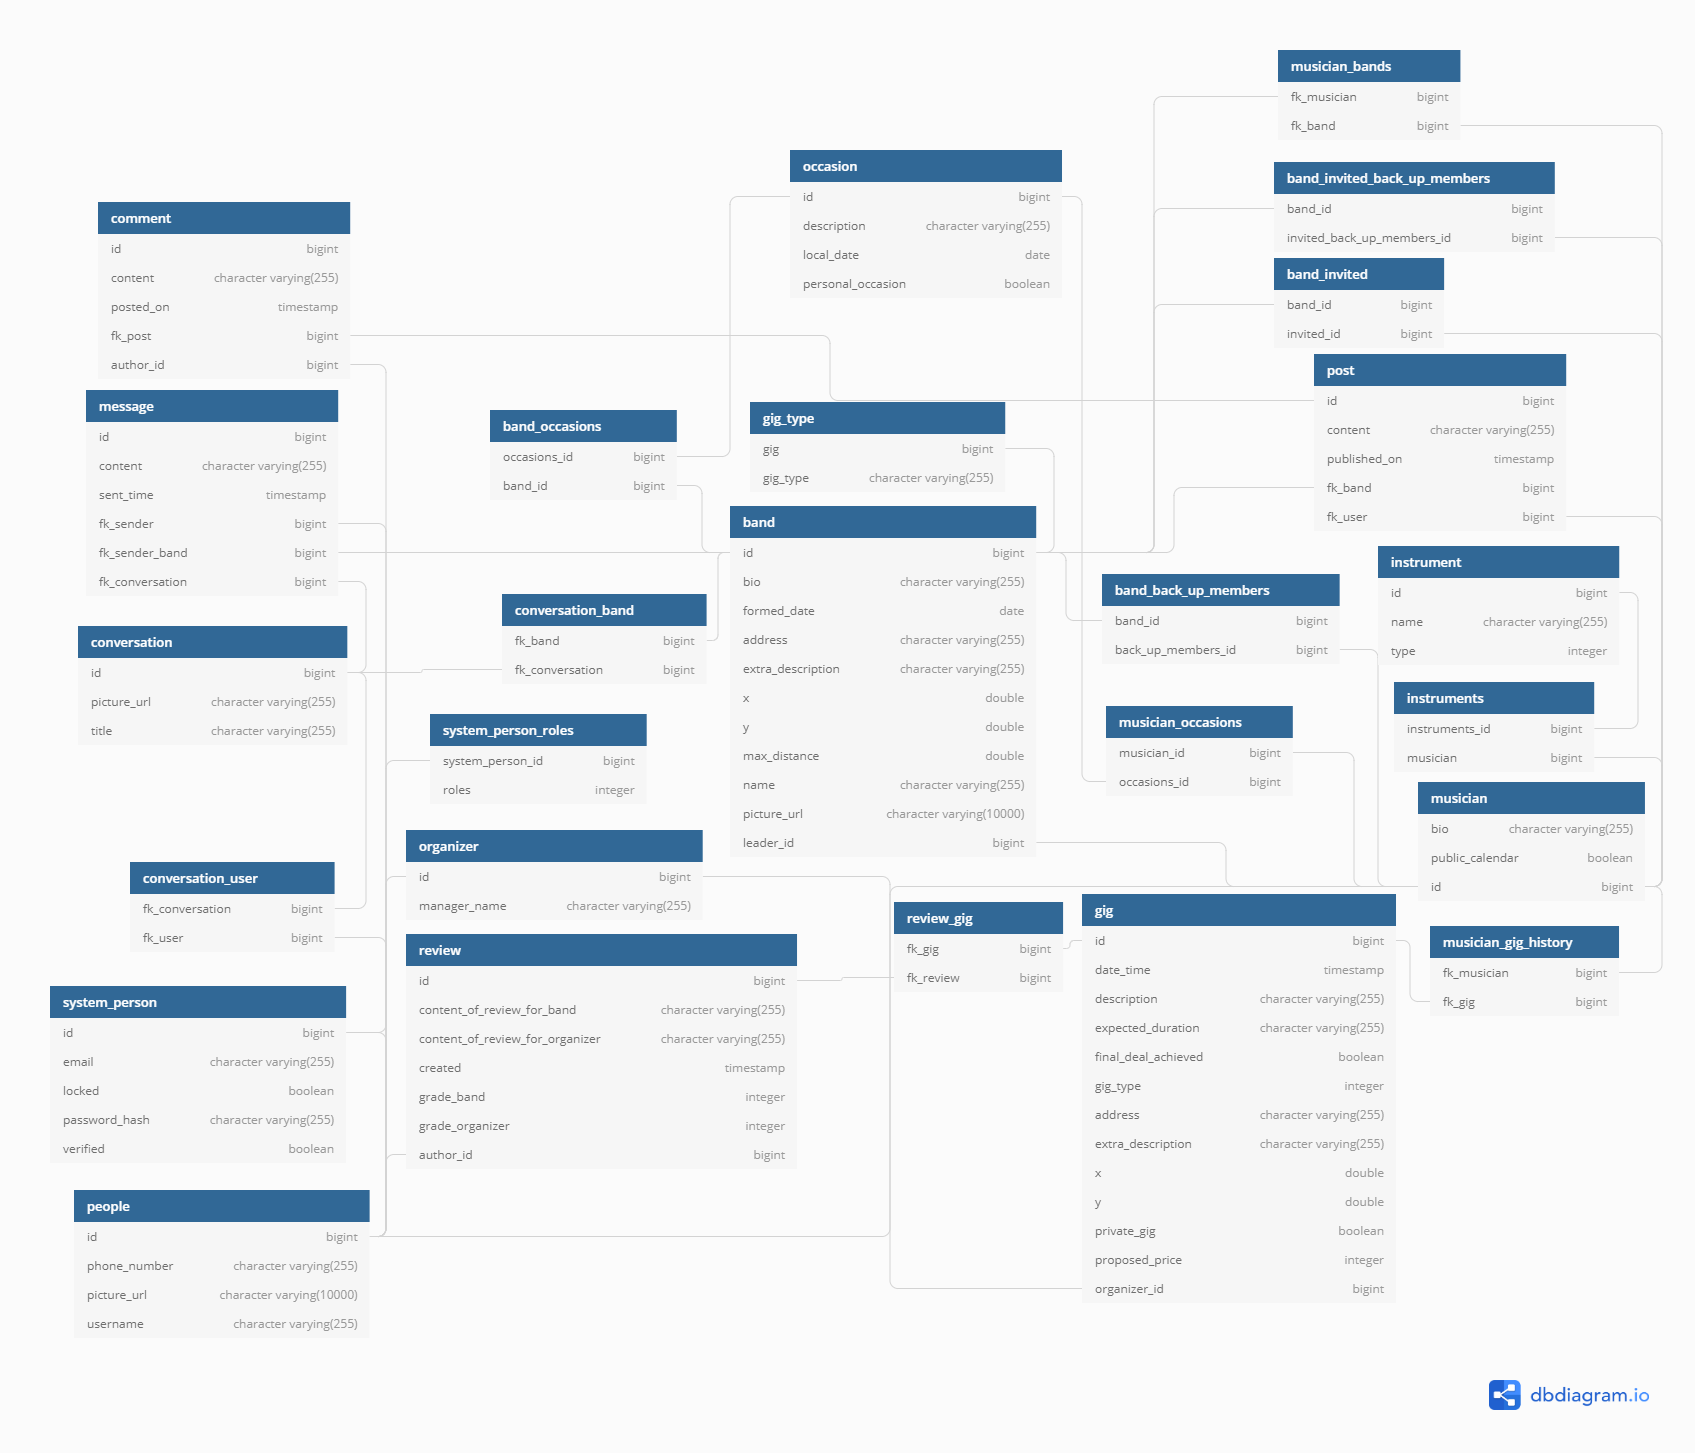
\includegraphics[width=17cm]{slike/ERModel.PNG}
			\end{center}
			\caption{Dijagram baze podataka}
			\label{fig:dijagramBaze}
		\end{figure}
			
			
			
		\section{Dijagram razreda}
		
			\textit{Potrebno je priložiti dijagram razreda s pripadajućim opisom. Zbog preglednosti je moguće dijagram razlomiti na više njih, ali moraju biti grupirani prema sličnim razinama apstrakcije i srodnim funkcionalnostima.}\\
			
			\textbf{\textit{dio 1. revizije}}\\
			
			\textit{Prilikom prve predaje projekta, potrebno je priložiti potpuno razrađen dijagram razreda vezan uz \textbf{generičku funkcionalnost} sustava. Ostale funkcionalnosti trebaju biti idejno razrađene u dijagramu sa sljedećim komponentama: nazivi razreda, nazivi metoda i vrste pristupa metodama (npr. javni, zaštićeni), nazivi atributa razreda, veze i odnosi između razreda.}\\
			
			\textbf{\textit{dio 2. revizije}}\\			
			
			\textit{Prilikom druge predaje projekta dijagram razreda i opisi moraju odgovarati stvarnom stanju implementacije}
			
			
			
			\eject
		
		\section{Dijagram stanja}
			
			
			\textbf{\textit{dio 2. revizije}}\\
			
			\textit{Potrebno je priložiti dijagram stanja i opisati ga. Dovoljan je jedan dijagram stanja koji prikazuje \textbf{značajan dio funkcionalnosti} sustava. Na primjer, stanja korisničkog sučelja i tijek korištenja neke ključne funkcionalnosti jesu značajan dio sustava, a registracija i prijava nisu. }
			
			
			\eject 
		
		\section{Dijagram aktivnosti}
			
			\textbf{\textit{dio 2. revizije}}\\
			
			 \textit{Potrebno je priložiti dijagram aktivnosti s pripadajućim opisom. Dijagram aktivnosti treba prikazivati značajan dio sustava.}
			
			\eject
		\section{Dijagram komponenti}
		
			\textbf{\textit{dio 2. revizije}}\\
		
			 \textit{Potrebno je priložiti dijagram komponenti s pripadajućim opisom. Dijagram komponenti treba prikazivati strukturu cijele aplikacije.}